% Hadron-Hadron Scatteing
%%%%%-------PROVA-------------
%\documentclass[12pt]{report}
%\usepackage[british]{babel}
%\usepackage{amsmath}
%\usepackage{amsfonts}
%\usepackage{amssymb}
%\usepackage{geometry}
%\geometry{hmargin={2cm,2cm},vmargin={2cm,2cm}}
%\usepackage{caption}
%\captionsetup{format=hang}
%\usepackage{graphicx}
%\usepackage{enumitem}
%\usepackage{float}
%
%
%
%\usepackage[colorlinks=true, linkcolor=blue]{hyperref} %to use autoref
%%%%%-------------------------

%\begin{document}


\chapter{Hadron-Hadron Scattering}
\label{chap:Hadron-HadronScattering}

In a high energy proton-proton collision we can have either soft or hard processes. Most of the time the hard processes are accompanied by soft interaction, occurring along the hadron interaction.
While, the hard processes as the Higgs boson production, the high $p_T$ jet production are well understood using perturbation theory, the soft processes as the underlying event, the hadronization are not so well understood. In fact, these processes are described by non perturbative QCD. 

This chapter gives a theoretical introduction on the QCD factorization theorem, the fixed order calculation for the perturbative approach and on the all orders approaches (e.g. the parton shower).

\section{QCD factorization theorem}

The fundamental idea for the description of a hadron-hadron collision is given by the fact that hadrons are made-up from partons that, at some high energy scale, can be seen as free. So the hadron-hadron interaction can be seen as an interaction between two free partons, given a sufficient high energy scale for the interaction.\\
This idea was developed in the framework of the deep inelastic scattering, and the Bjorken scaling observation confirms it \cite{Bjorken:1968dy}. The generalization of this concept leads to the QCD factorization theorem. 
   
The factorization theorem was introduced first by Drell and Yan \cite{DRELL1971578}. 
The hadron-hadron scattering is described in terms of partons extending the formalism used for deep inelastic scattering 
\begin{equation}
\sigma_{AB}=\displaystyle\int dx_a\,dx_b\,f_{a/A}(x_a)\,f_{b/B}(x_b)\,\hat{\sigma}_{ab \rightarrow X}\quad .
\label{eq:factorization1}
\end{equation}
Where X is a partonic/leptonic state and $a\,(b)$ a quark or an antiquark in the hadron $A\,(B)$. This is valid in the "scaling" limit:
\begin{equation}
	s\ \longrightarrow\ \infty\ , \qquad\qquad\qquad \frac{M_X}{\sqrt{s}}=\text{finite}\quad ;
\end{equation}
where the center-of-mass energy grows to infinity but with a fixed ratio of the X state invariant mass and the center-of-mass energy.

The problem arises from the perturbative corrections from real and virtual gluon emission, in particular from the colinear gluon emissions. These contributions take to a logarithmic divergence (spoil the convergence of the perturbative expansion). These dependencies can be absorbed by the parton distribution functions (DGLAP equations). This results in the violation of the scaling 
\begin{equation}
	f_{a/A}(x_a)\ \longrightarrow\ f_{a/A}(x_a, Q^2)\quad , 
\end{equation}  
now, the parton distribution function depend on the momentum scale $Q^2$ of the interaction. 

So, we can rewrite the factorization theorem in \eqRef{eq:factorization1} as:
\begin{equation}
	\sigma_{AB}=\displaystyle\int dx_a\,dx_b\,f_{a/A}(x_a,Q^2)\,f_{b/B}(x_b,Q^2)\,\hat{\sigma}_{ab \rightarrow X}\quad ,
\label{eq:factorization2}
\end{equation}
at this point the \emph{finite} corrections to the leading-logarithmic cross section in the perturbative expansion are specific for each process (not universal, they are process dependent). This leads in the \eqRef{eq:factorization2} to the $\alpha_s$ series:
\begin{equation}
	\sigma_{AB}=\displaystyle\int dx_a\,dx_b\,f_{a/A}(x_a,\mu_F^2)\,f_{b/B}(x_b,\mu_F^2)\,\left[\hat{\sigma}_0+\alpha_s(\mu_R^2)\hat{\sigma}_1+\dots\right]\quad .
\label{eq:factorization3}
\end{equation}
In \eqRef{eq:factorization3} two scales enter the formula:
\begin{itemize}
	\item[--] The \textit{factorization scale} $\mu_F$: this scale separates long- and short- distance physics, this scale is related to the resolution with which the hadron is being probed.
	\item[--] The \textit{renormalization scale} $\mu_R$: the scale at which is evaluated the strong coupling constant $\alpha_s$. The dependence of $\alpha_s$ on the renormalization scale is related to different effects such as  the vacuum polarization, the quark self-energy, the vertex corrections, and the gluon loop corrections to the elementary three-gluon and four-gluon couplings.
\end{itemize}

The higher-order corrections to the cross section in \eqRef{eq:factorization3} are important because they lead to an improvement in the cross section prediction, gradually reducing the dependencies on $\mu_R$ and $\mu_F$. In the absence of an all order prediction, a choice for the two scales have to be taken.
Typically, the scales are assumed to be equal: in the Drell-Yan process the standard choice is $\mu_F=\mu_R=M$, with $M$ the lepton pair mass \cite{Campbell2006}; other cases are the invariant masses of $Z$-boson and top quark or the jet transverse energy to study \cite{Campbell2006} the production cross sections for Z-bosons, top quarks and large $E_T$ jets.

The parton distribution functions used in the hard scattering are solution to the DGLAP (Dokshitzer–Gribov–Lipatov–Altarelli–Parisi) equation \cite{Lipatov:400357, Gribov:427157, ALTARELLI1977298, Dokshitzer:1977sg}
\\
\begin{equation}
	\mu_F^2\frac{\partial f_{i/H}(x,\mu_F^2)}{\partial\mu_F^2}=\displaystyle\sum_j\frac{\alpha_s(\mu_F^2)}{2\pi}\displaystyle\int_x^1 \frac{dz}{z}\, P_{i\,\rightarrow\,j}(z)\ f_{j/p}\left(\frac{x}{z},\mu_F^2\right)\quad .
\end{equation}
\\
Where $P_{i\,\rightarrow\,j}$ are the splitting functions: they are the probability to have a parton of type $i$ that becomes, by the emission of a quark or a gluon, a parton $j$, carrying fraction $z$ of the momentum of parton $i$.
\\
The splitting functions have perturbative expansions: 
\begin{equation}
	P_{i\,\rightarrow\,j}(x,\alpha_s)=P_{i\,\rightarrow\,j}^{(0)}(x)+\frac{\alpha_s}{2\pi}P_{i\,\rightarrow\,j}^{(1)}(x)+\dots\quad .
\end{equation}
\\
This procedure has been used to calculate Standard Model cross section in $p\overline{p}$ and $pp$ scattering respectively at Tevatron and LHC energies as shown in \figRef{figure:StandardModelCrossSections}.

\begin{figure}[!ht]
	\centering 
	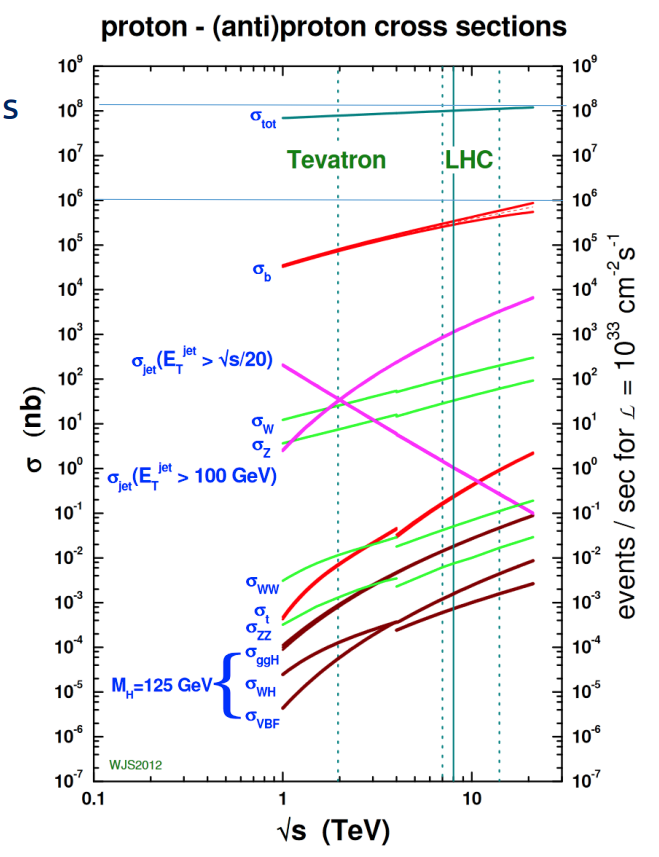
\includegraphics[width=12cm]{img/StandardModelCrossSections_color.png}
	\caption{Next-to-leading order cross sections at Tevatron and LHC colliders energies (the splitting are at the transition between $p\overline{p}$ and $pp$ cross section). Figure from \cite{StirlingPrivate}}
	\label{figure:StandardModelCrossSections}
\end{figure}

The parton distribution functions dependence on $Q^2$ can be derived theoretically via the DGLAP equations. While, the $x$ dependence is given fitting the deep-inelastic and other hard-scattering processes experimental data.
The experimental coverage in $(x,Q^2)$-plane is shown in \figRef{figure:xQ2planeCoverage} 
where is also underlined the relationship between $(x,Q^2)$ and kinematic variables in Drell-Yan processes for a final state with invariant mass $M$ and rapidity $y$ is shown, further details in section 2 of \cite{Campbell2006}. Assuming that the factorization scale $Q$ is equal to $M$ (The reference center of mass energy is $13\ \mathrm{TeV}$), for two incoming particles with four-momentum respectively $p_1$ and $p_2$ the relations with $y$ and $M$ are:  
\begin{equation}
	\begin{aligned}
		&p_1^\mu=\frac{\sqrt{s}}{2}(x_1,0,0,x_1)\\
&p_2^\mu=\frac{\sqrt{s}}{2}(x_2,0,0,-x_2)
	\end{aligned} \quad\Longrightarrow\quad x_1=\frac{M}{\sqrt{s}}e^y\qquad x_2=\frac{M}{\sqrt{s}}e^{-y} \quad ,
\end{equation}
where  $s=(p_1^\mu+p_2^\mu)^2$. For example the figure shows that the production of a final state with invariant mass $M=100\ \mathrm{GeV}$ and rapidity $y=2$ is given by the interaction of two hadrons with $x_1\approx0.05$  and $x_2\approx0.001$ with $Q^2=10^4\ \mathrm{GeV^2}$


\begin{figure}[!ht]
	\centering 	
	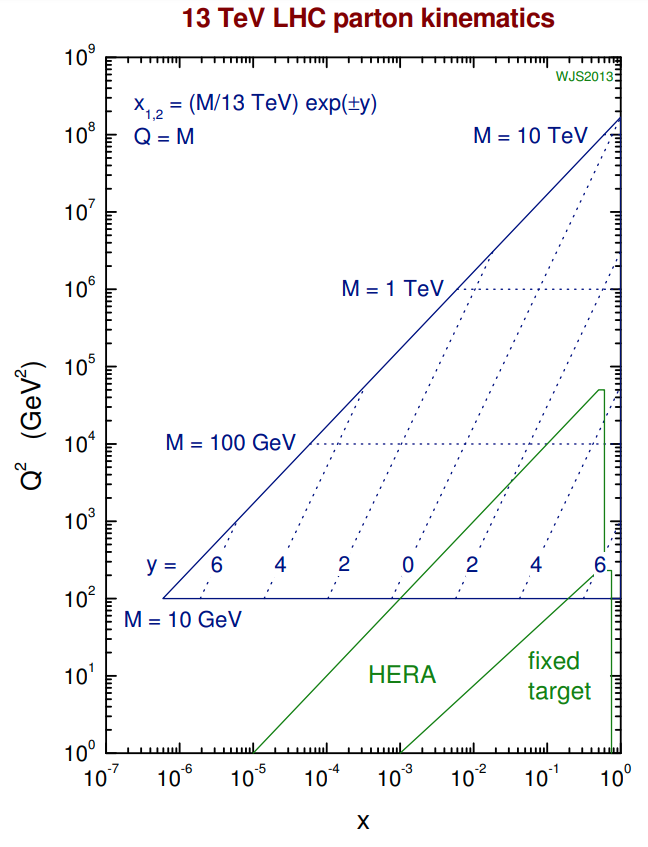
\includegraphics[width=12cm]{img/xQ2planeCoverage.png}
	\caption{Graphical representation of the parton $(x,Q^2)$ variables coverage of different experiments. For LHC these $x$ and $Q^2$ are related to the kinematic variables $y$ and $M$. Figure from \cite{StirlingPrivate}}
		\label{figure:xQ2planeCoverage}
\end{figure}

\section{Partonic cross section}

Partonic cross section is one of the fundamental ingredients in our recipe for the description of hadron-hadron interactions. This can be calculated in a perturbative series in $\alpha_s$ from QCD first principles using quantum field theory.
\\
The calculation at the leading order (LO) is performed evaluating all the possible tree-level Feynman diagrams for every process. Than the calculation proceeds computing the squared matrix element and integrating over the available phase space (analytically or numerically).
\\
At this point, we can already encounter some divergence that have to be avoided imposing restrictions on the phase space.
% restriction or constraints

\subsection{Higher order calculations}

The LO calculation can describe broad feature of a particular process and provide a first estimation of its cross section; anyway, in many cases this is insufficient.
\\
The main source of uncertainty derives from the LO dependence  on the unphysical renormalization and factorization scales. Some process may contribute only when going beyond the first approximation, and some divergence can be resummed. 
\\
To the next-to-leading order (NLO) calculation requires all the Feynman diagrams that take an extra $\alpha_s$. This contribution can arise in two different ways:
\begin{itemize}
	\item Virtual: internal lines (loops);
	\item Real: external lines (real particles).
\end{itemize}
Virtual corrections contains infrared divergences, arising from the integral on the loop circulating momentum, that cancel against infrared singularities given by collinear emissions or soft emissions \cite{PhysRevBloch, KinoshitaToichiro, PhysRevLee}. 
\\
A common strategy for the renormalization is dimensional regularization: it consists into performing the calculation in a $D=4-2\epsilon$-dimensional space ($\epsilon<0$), in that way the singularities appear as single and double poles in $\epsilon$. Than, the limit $\epsilon\rightarrow0$ is taken after the divergences have cancelled.
\\
This NLO calculation with regularization allows to extend the treatment to zero transverse momentum.

The importance of higher order calculations can be seen with the following example. In a $Z$ boson production:
\begin{enumerate}[label=$\arabic*)$]
	\item \textbf{LO}: the $Z$ is produced without transverse momentum ($p_T$), anything can recoil against the $Z$ for momentum conservation (\figRef{fig:Zprod_feynman_LO_NLO_NNLO}{\color{blue}{a}}). 
	\item \textbf{NLO}: the $Z$ acquire a finite $p_T$, in this case the $Z$ boson $p_T$ is balanced by a single \mbox{parton/gluon} (\figRef{fig:Zprod_feynman_LO_NLO_NNLO}{\color{blue}{b}}).
	\item  \textbf{NNLO}: the $Z$ $p_T$ can be balanced by two jets (\figRef{fig:Zprod_feynman_LO_NLO_NNLO}{\color{blue}{c}}). 
\end{enumerate}
\begin{figure}[!ht]
 \centering
 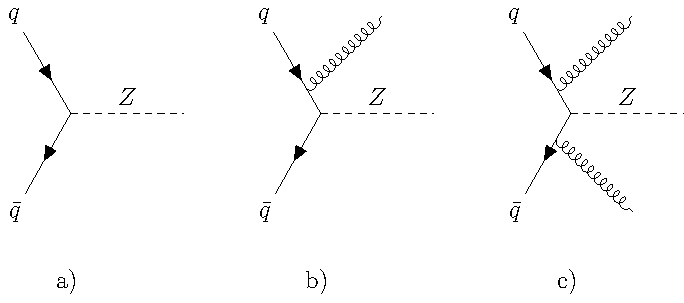
\includegraphics[width=12cm]{{img/feynman_ZpT.pdf}}
 \caption{Feynman diagrams for the Z production by annihilation of a quark and an antiquark at LO (a), NLO (b), NNLO (c). At LO the $Z$ can only be produced with a $p_T=0$ for the conservation of the momentum.}
 \label{fig:Zprod_feynman_LO_NLO_NNLO}
\end{figure}
Another important benefit of performing a NLO calculation is the the reduction of the dependence on the unphysical renormalization ($\mu_R$) and factorization ($\mu_F$) scales.
It is proven that higher order calculations of observables calculated to order $\alpha_s^{\,n}$ are dependent on the unphysical scales only at order higher than $\alpha_s^{\,n+1}$ \cite{Campbell2006}. The range of predictions corresponding to different scale choices is usually attributed to \textit{theoretical uncertainties}, this is shown in \figRef{fig:ZRapidityDistributionLO_NLO_NNLO}, where the uncertainties reduce from the LO calculation to the NLO and even more to the NNLO.

\begin{figure}[!ht]
	\centering
	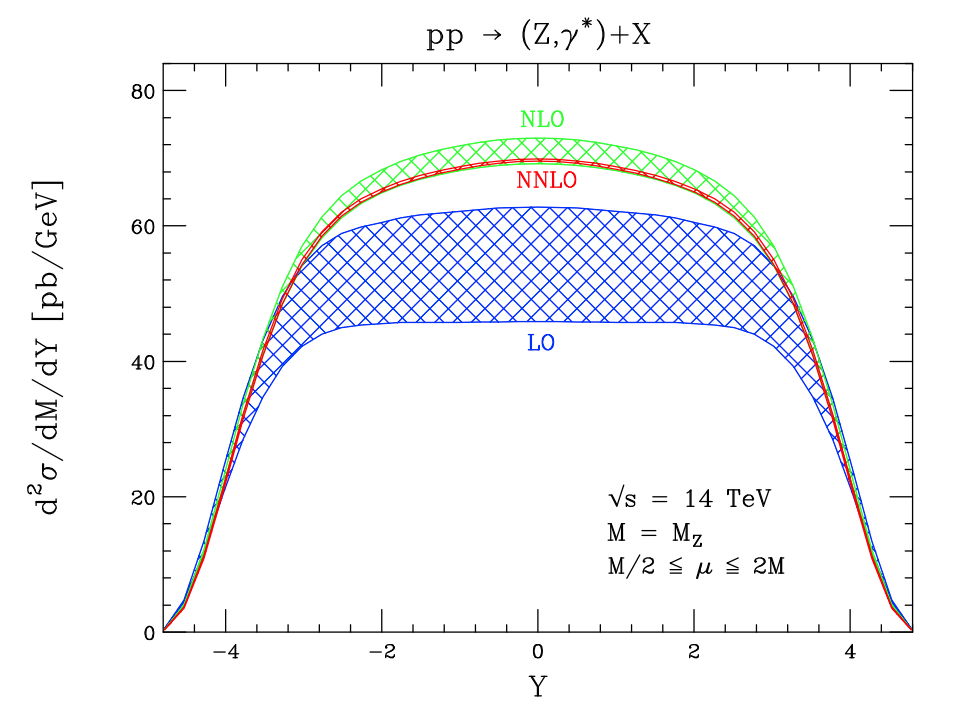
\includegraphics[width=12cm]{{img/ZRapidityDistributionLO_NLO_NNLO.png}}
	\caption{The rapidity distribution predictions at LO (blue) NLO (green) and NNLO (red) for the Z production at the center of mass energy$\sqrt{s}=14\ \mathrm{TeV}$. The band width is related to the uncertainties. Going from LO to NLO there is a increase in the cross section prediction and a reduction on the scales uncertainties, the NNLO prediction is in the NLO error band width but there is a further increase in the precision of the prediction. Figure from \cite{Campbell2006}, section 6.}
	\label{fig:ZRapidityDistributionLO_NLO_NNLO}
\end{figure}

\section{Parton Showers}

A different approach, instead than calculating order by order in the perturbative expansion, is the use of an \textit{all-order} approach to describe the phenomena observed at high-energy colliders. 
\\
Different all-order approaches exist such as resummation and parton showers. Resummation is based on the observation that in many quantities the smallness of the expansion coefficients $\alpha_s$ is violated by large logarithmic enhancements. This takes the dominant contribution from each order and "resums" them by means of an evolution equation. 
The main problem in QCD is related to the fact that lot of quantities have correction of the form $\alpha_s^n\log^k(Q_i/Q_j)$ where $Q_i$ and $Q_j$ are two different energies scales, for example:
\begin{itemize}
	\item[--] Renormalization and factorization scales logs: $\alpha_s^n\log^n(Q^2/\mu_f)$
\end{itemize}
Various methods to perform this resummation exist.
\\
%%%% GRAPH on pT Z with effect of resummation 
An example is the $Z$ production $p_T$ spectrum shown in \figRef{figure:pT_Z_CDF}: here the comparison between experimental CDF data and theoretical predictions is shown: in the low $p_T$ region the \textit{all-order} approach regularizes the divergence of the fixed order calculation and describes the data better. 

\begin{figure}[!ht]
	\centering
	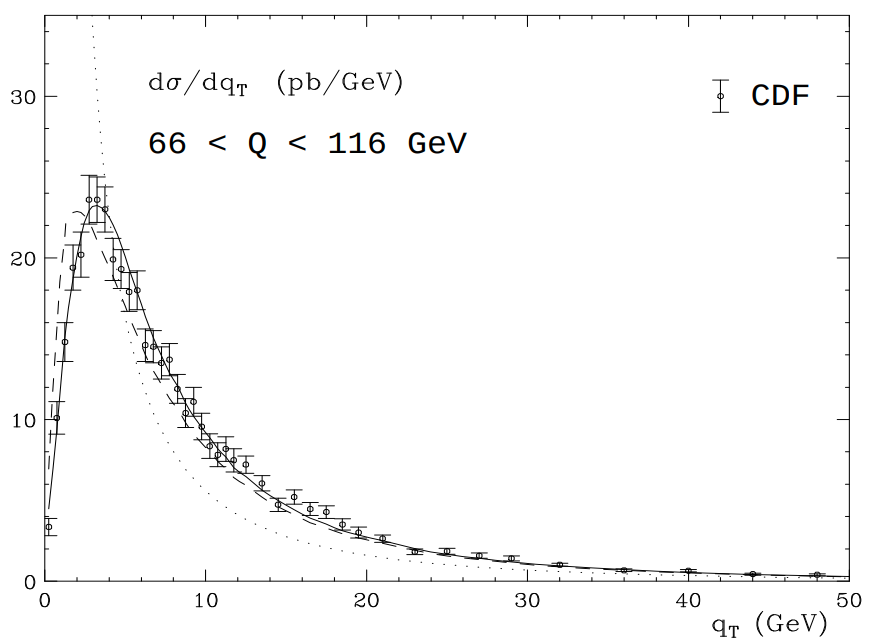
\includegraphics[width=12cm]{{img/pT_Z_CDF.png}}
	\caption{CDF data on $Z$ production cross section at Tevatron collider, CDF experiment, the predictions from fixed order calculation (dotted) with resummation (dashed), and with the inclusion of power corrections (solid) are compared. Figure take from \cite{kulesza2002electroweak}}
	\label{figure:pT_Z_CDF}
\end{figure}

An other \textit{all-order} approach is parton showers: it is  implemented in different programs, as  \textsc{pythia} \cite{PYTHIA2015}, \textsc{herwig} \cite{Herwig2008} and \textsc{sherpa} \cite{SHERPA2004}. This starts from few parton arising from hard interaction and than these are related to partons to a lower energy scale close to $\Lambda_{QCD}$ using the DGLAP evolution equation formalism. The solution to this equation can be written using a Sudakov form factor arising from the probability of no gluon emission in the evolution from higher scale to lower scale.
\\
In the parton showering process, additionally to the kinematic variable (momentum fraction $z$ and an azimuthal angle $\phi$) and flavours of the partons, an evolution variable $t$ is generated.\textsc{Pythia8} use as  evolution variable the squared of the relative transverse momentum of the two partons in the splitting ($p_T^2$). Different choices are made in \textsc{herwig} and \textsc{sherpa}.
\\
As mentioned before, the shower evolution is based on the standard (LO) DGLAP splitting kernels P(z) described here:
\begin{align}
P_{q\,\rightarrow\,qg}(z) & = C_F\frac{1+z^2}{1-z}\quad ; \\
P_{g\,\rightarrow\,gg}(z) & = C_A\frac{(1-z(1-z))^2}{z(1-z)}\quad ; \\
P_{q\,\rightarrow\,q\overline{q}}(z) & = T_R(z^2+(1-z)^2)\quad ;
\end{align} 
where $C_F=\frac{4}{3}$, $C_A=N_C=3$ and $T_R=\frac{1}{2}$, each contribution is multiplied by $N_f$ if summing over all contributing quark flavours.
\\
Both Initial State Radiation (ISR) and Final State Radiation (FSR) algorithms are based on these splitting kernels.
The respective probabilities of emitting radiation as one moves in the decreasing evolution variable sequence are:
\begin{align}
	FSR: \qquad\quad & \frac{d\mathcal{P}_{FSR}}{dp_T^2} = \frac{1}{p_T^2}\displaystyle\int \frac{dz}{z}\,\frac{\alpha_s}{2\pi}P(z)\quad ;\label{eq:FSR1}\\
	ISR: \qquad\quad & \frac{d\mathcal{P}_{ISR}}{dp_T^2} = \frac{1}{p_T^2}\displaystyle\int \frac{dz}{z}\,\frac{\alpha_s}{2\pi}P(z)\,\frac{f'(x/z,p_T^2)}{f(x,p_T^2)}\quad .\label{eq:ISR1}
\end{align}
We can write-out our Sudakov form factor by using the two probability in \eqRef{eq:FSR1} and \eqRef{eq:ISR1}, as
\begin{equation}
	\Delta(p_T^2)=\exp\left( -\displaystyle\int_{p_T0}^{p_T'} \frac{d\mathcal{P}_{PS}}{dp_T^2} \,dp_T\right) \qquad\text{ with } \quad PS=ISR,\ FSR \quad.
	\label{eq:sudakovFormFactor}
\end{equation}
The Sudakov form factor give the probability of a parton to evolve from an harder scale to a softer scale without emitting a parton harder than some resolution scale. 
\\
The introduction of the Sudakov form factor resums all the effects from the soft and collinear gluon emission. For more details and some plots of different Sudakov form factor values see section 3.5 of \cite{Campbell2006}.

\subsection{Merging parton showers and matrix element calculations}

What we have now is: regions dominated by soft and collinear gluon emissions are described very well by parton showers approach; on the other hand, regions where partons are  energetic and widely separated are well described by matrix element calculations.  
So, the best approach would be to combine the two different description, This would require an universal formalism for parton showers and matrix element calculations. This universal formalism was created in 2001 and it is call "Les Houches Accord" \cite{LesHouchesAccord}.
In order to combine the two approach some care must be taken: there is the risk of double counting. There are different technique that prevent this risk for example CKKW \cite{CKKW2001} is used to combine LO matrix element calculations and parton shower.


A more best way is to combine NLO matrix element calculation with parton showers this is done by Frixione, Nason, Webber in the \textsc{mc@nlo} framework \cite{FxFx1,FxFx2,FxFx3,FxFx4}. In this scenario the risk of  double counting is given by the fact that at NLO one emission is made real, than the progress of the parton shower give a double counting between real and virtual emission as shown in \figRef{fig:DoubleCounting}.
% TODO: mi piacerebbe aggiungere una descrizione più completa del merging con FxFx visto che viene usato dopo. 

%%%
%%% Immagine di Frixi.. presentation
\begin{figure}[H]
	\centering
	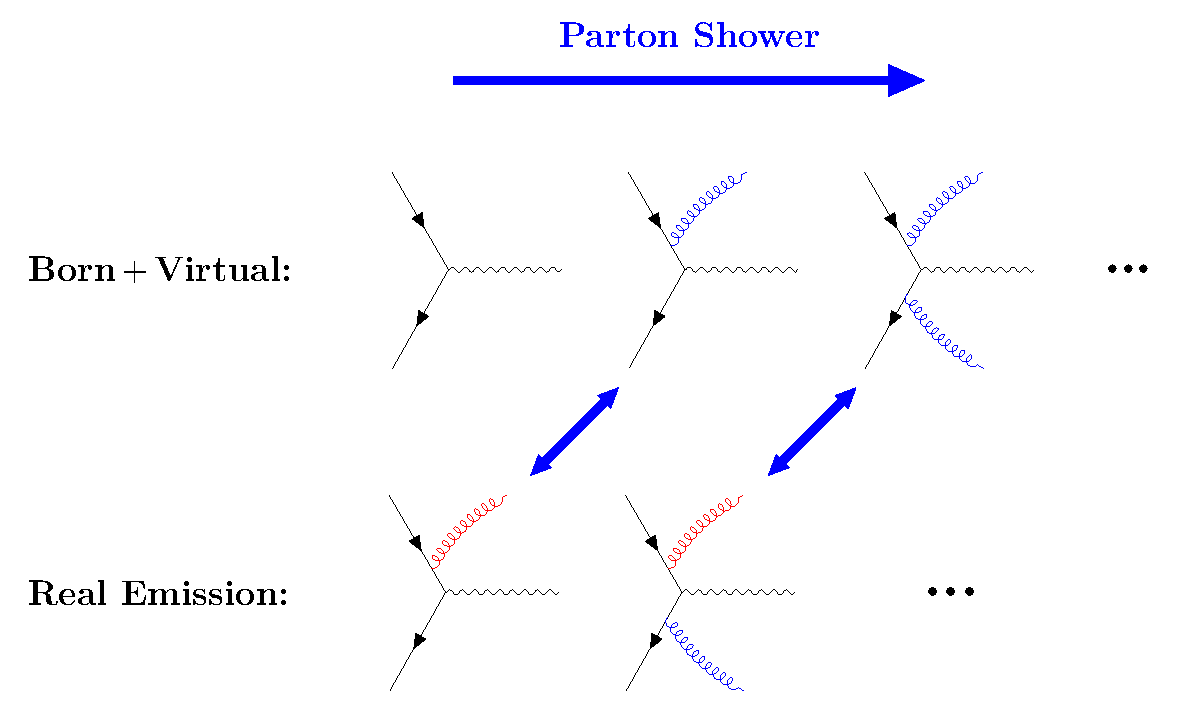
\includegraphics[width=14cm]{{img/feynman_doubleCounting_FxFx_curved-cropped.pdf}}
	%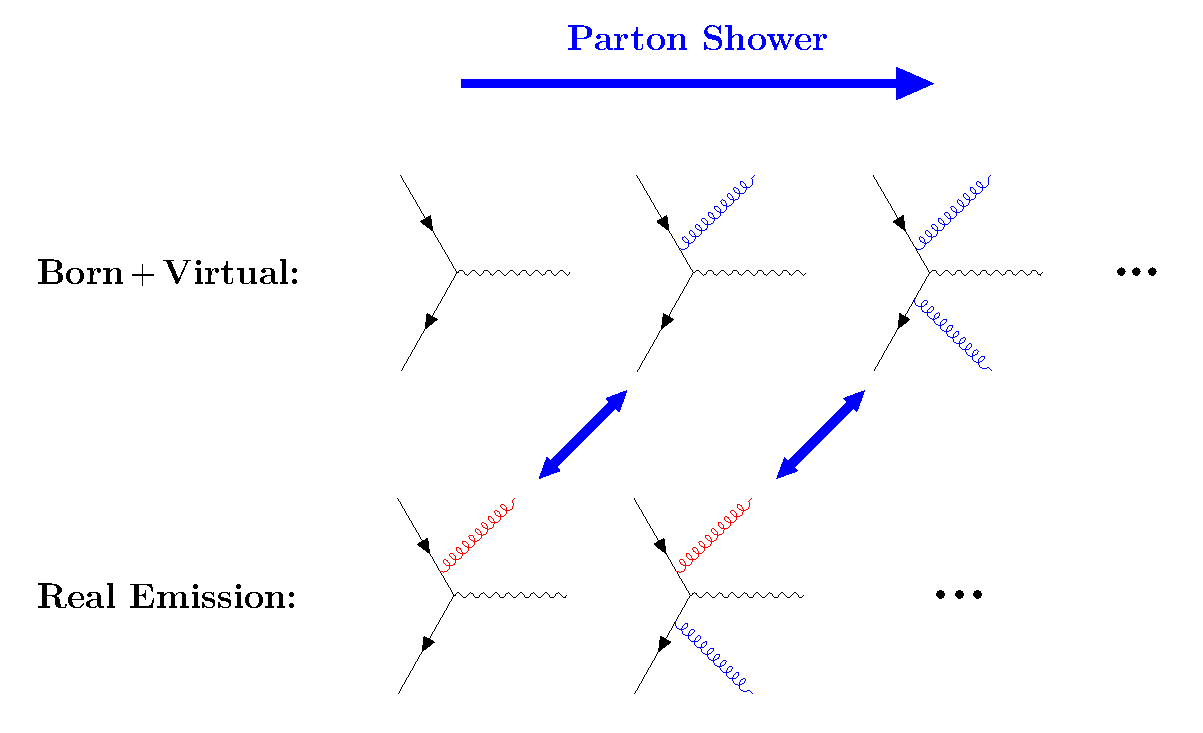
\includegraphics[width=14cm]{{img/feynman_doubleCounting_FxFx-cropped.pdf}}
	\caption{The FxFx margin scheme have to avoid this double counting. Feynman diagrams that can lead to a double counting are grouped with the violet arrow, the blue emission are related to the parton shower while the red ones to the NLO process.}
	\label{fig:DoubleCounting}
\end{figure}
%%%


\section{Parton distribution functions}

The last ingredient in our recipe is the knowledge of the quark and gluon distributions inside the two hadrons that undergo to the scattering. We have already seen that these quantities are depending on the virtuality of the interaction.
\\
The information on the quark distribution inside a hadron $f_{q/p}(x,Q^2)$ arises from lepton-hadron DIS experiments, from lepton-pair production in hadron-hadron collisions (Drell-Yan processes) and jet measurements to study gluon distribution $f_{g/p}(x,Q^2)$. All these quantities are the experimental input in order to evaluate the PDF inside the hadron while the $Q$-evolution can be described by DGLAP equation.
The evolution of the PDF can be run either with a NLO or with a NNLO calculations.

The kinematic region covered by experiments is shown in \figRef{figure:xQ2planeCoverage}. At very low x and $Q^2$ the DGLAP evolution is believed to be no longer applicable and a BFKL (Balitsky-Fadin-Kuraev-Lipatov) \cite{BFKL1,BFKL2} description must be used;
anyway, this has not any experimental evidence so the DGLAP approach is used as default in all the PDF analysis.
% but there are no experimental evidence of this so the DGLAP approach is used as default in all the PDF analysis.
\\
A lot of processes are available for the PDFs evaluation and a lot of PDF set have been generated, as an example \figRef{fig:NNPDF31} shows the NNPDF3.1 set \cite{NNPDF3.1} at NNLO for a virtuality $Q^2=10\ \mathrm{GeV^2}$ (left) and $Q^2=10^4\ \mathrm{GeV^2}$ (right). 
\begin{figure}[!ht]
	\centering
	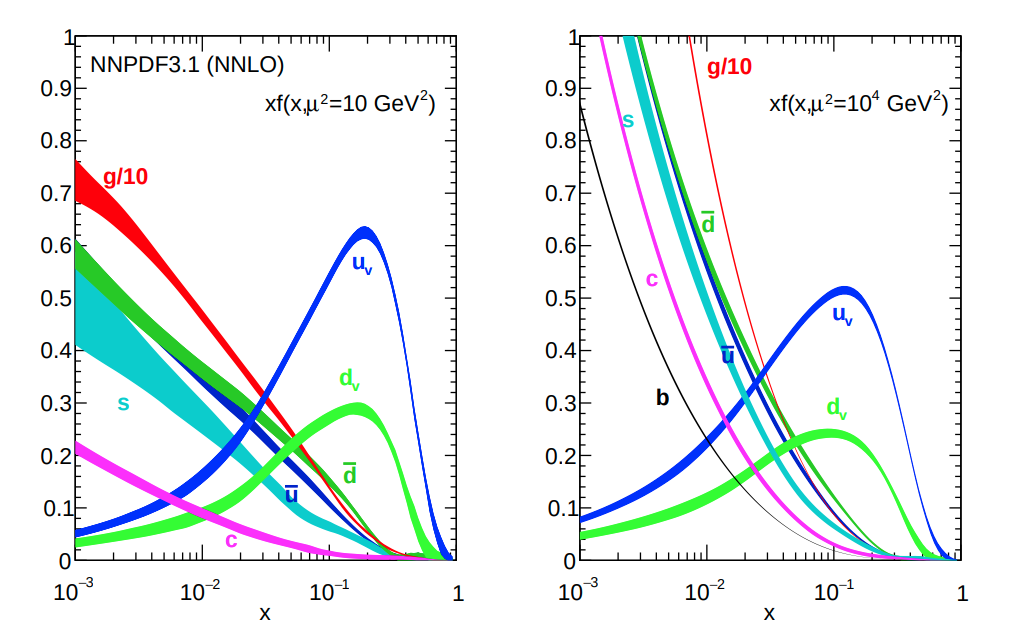
\includegraphics[width=12cm]{{img/NNPDF3.1.png}}
	\caption{The NNPDF3.1 NNLO PDFs set, evaluated at $Q^2 = 10\ \mathrm{GeV}^2$
(left) and $Q^2=10^4\ \mathrm{GeV}^2$ (right). At low $x$ the contribution from the gluons is the dominating one while at higher x the dominant contribution is from the valence quarks. The PDF $Q$ evolution shows that when our proton is probed to higher $Q^2$ the resolution increase (higher $Q$ correspond to smaller distance resolution) and so we have a bigger contribution from the sea quarks at low $x$ values.}
	\label{fig:NNPDF31}
\end{figure}
Note that the gluon contribution have been scaled of a factor 10: in fact, in the low $x$ region, $x<0.01$, the gluon contribution is the dominating one, while at high $x$ value the valence quarks dominate the PDF. 
\\
In \figRef{fig:NNPDF31} we can also see that with increasing virtuality ($Q^2$) at low $x$ the density of the sea quarks increases: this is related to the fact that our hadrons are probed at higher energy and the probe resolution is proportional to the energy. 
\begin{equation}
	\text{Resolution}\sim\frac{\hbar}{Q}\quad .
\end{equation}
So, when probed at higher energy, the hadrons appear denser than when are probed at lower energy. This, as will be discussed in the next chapter, is related to the higher number of interaction between partons in a single hadron-hadron collision. The phenomenon of having more than one interaction between partons in a single hadron-hadron collision is called \textit{multiple parton interaction}: this concept will be discussed in the next chapter.


\section{A real proton-proton collision}


We have understood that the complexity in the description of a proton-proton collision arises from composite nature of the protons. In this chapter we discussed the importance of the QCD factorization theorem that help us in the calculation of the hadronic cross section with the convolution between the partonic cross section and the PDF. We have discussed the importance of the parton shower algorithm where a set of partons are evolved in a more complex final state by emissions in the initial and final states.
\\
All these processes are important in the description of a real proton-proton collision but also the partons that are left unscattered are non-color singlet and can contribute to the complex final state observed in the experiments, and additionally, as mentioned before, nothing prevent additional partons scatterings from taking place and growing more and more the complexity of the partons final state. 

Than, another problem is related to the not-well-understood hadronization process.
Hadronization is not known from first principles and different models have been implemented in different programs: the \textit{cluster fragmentation model} implemented in \textsc{herwig} and the \textit{string fragmentation model} in \textsc{pythia} simulated this process of hadronization where the set of final-state partons is transformed into a set of hadrons. All these processes are schematically shown in \figRef{fig:Processes}.

\begin{figure}[!ht]
	\centering
	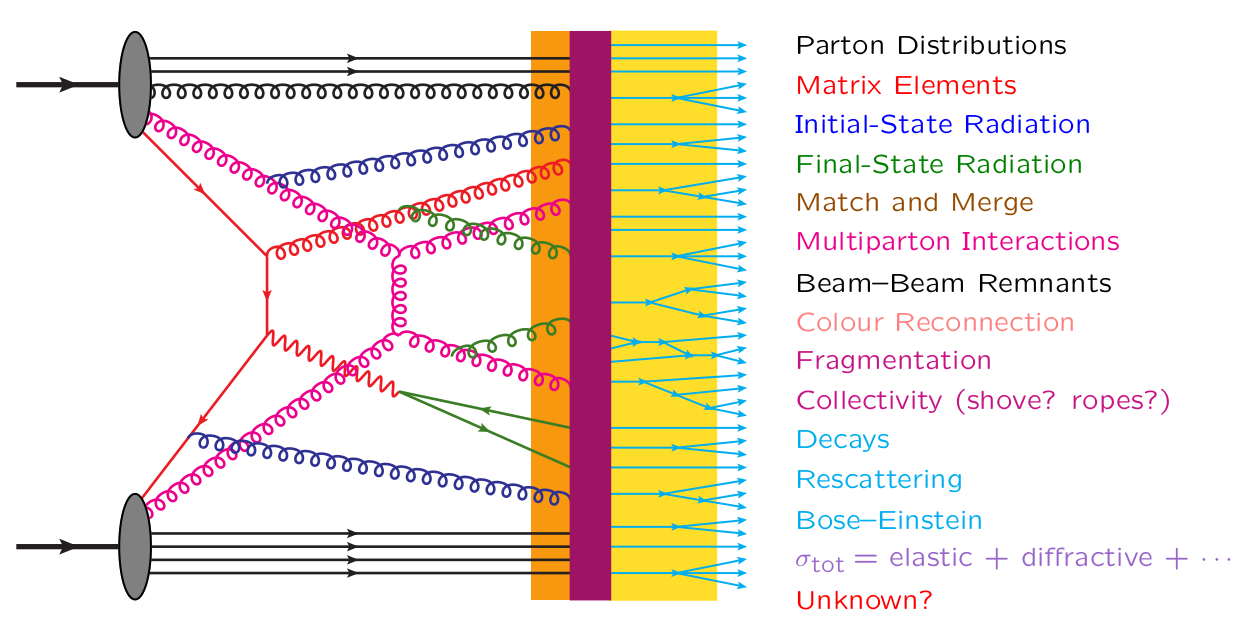
\includegraphics[width=0.98\textwidth]{{img/Processes.png}}
	\caption{A schematic representation for a $pp$ collision. Reading the image from left to right one can have an idea on the evolution of the system. The two incoming hadrons enter the scattering from the left side, the read line indicate the main hard scattering and the fuchsia one the second parton scattering (MPI) each interaction is associated with initial (blue) and final (green) state radiation, the unscattered partons (black lines) re-enter the color reconnection and hadronization processes. Than the new formed hadrons (lightblue) can undergo to different decays.}
	\label{fig:Processes}
\end{figure}

Next chapter is going to describe the \textsc{pythia} Monte Carlo generator in more details. \textsc{pythia} introduces different free parameters that need to be tuned with experimental data from Tevatron and LHC. The tune methods are described in \chapRef{chap:TuneprocedureCP5TuneandMCNNTUNES} along with the description of some already existing tune for the underlying event in proton-proton collision.



%%% ---



%In a \textbf{proton-proton collision}, additionally to the main hard scattering that can be described performing Matrix Element calculations (MEs) , also other scattering processes are possible. To well understood the proton-proton collision we need to describe other processes, besides to the hard scattering, that can underlying to this  \textbf{Multi Parton Interaction} (MPI) and the \textbf{Beam-Beam Remnants} (BBR).




%\end{document}